\documentclass[conference]{IEEEtran}
% Compile on Overleaf with pdfLaTeX + BibTeX (see NOTES.md).

\usepackage{cite}
\usepackage{amsmath,amssymb}
\usepackage{graphicx}
\usepackage{array}
\usepackage{booktabs}
\usepackage{url}
\usepackage{xcolor}
\usepackage{tikz}
\usetikzlibrary{arrows.meta,positioning,calc}

% Clearly marked placeholder (red) for details the authors must fill in.
\newcommand{\placeholder}[1]{\textcolor{red}{[#1]}}

\begin{document}

\title{From Static Retrieval to Granularity-Aware Search Policies: A Review of Agentic Retrieval-Augmented Generation with a Case Study on Live Workspace Data}

\author{
\IEEEauthorblockN{Ajit Paraskar}
\IEEEauthorblockA{\textit{Dept. of Computer Engineering}\\
\textit{Dr. D. Y. Patil Institute of Technology}\\
Pimpri, Pune, India\\
\placeholder{EMAIL: Ajit Paraskar}}
\and
\IEEEauthorblockN{Harshvardhan Patil}
\IEEEauthorblockA{\textit{Dept. of Computer Engineering}\\
\textit{Dr. D. Y. Patil Institute of Technology}\\
Pimpri, Pune, India\\
\placeholder{EMAIL: Harshvardhan Patil}}
\and
\IEEEauthorblockN{Prathamesh Kumbhar}
\IEEEauthorblockA{\textit{Dept. of Computer Engineering}\\
\textit{Dr. D. Y. Patil Institute of Technology}\\
Pimpri, Pune, India\\
\placeholder{EMAIL: Prathamesh Kumbhar}}
\and
\IEEEauthorblockN{Bikram Ghosh}
\IEEEauthorblockA{\textit{Dept. of Computer Engineering}\\
\textit{Dr. D. Y. Patil Institute of Technology}\\
Pimpri, Pune, India\\
\placeholder{EMAIL: Bikram Ghosh}}
}

\maketitle

\begin{abstract}
Retrieval-augmented generation (RAG) grounds large language models (LLMs) in external text, but the classic retrieve-once pipeline struggles with multi-hop questions, noisy context and data that changes over time. Agentic RAG addresses these problems by letting the model plan, search repeatedly, choose tools, critique its own evidence and keep memory across sessions. This paper reviews agentic RAG around one recent anchor work, GRASP, which trains a small policy model with reinforcement learning to coordinate semantic search, keyword search and on-demand paragraph reading over a sentence-level index. We organise the literature into a taxonomy of eight design dimensions: query planning, iterative and adaptive retrieval, search granularity and search policies, self-reflection and corrective retrieval, tool use and connector protocols, long-term memory, attribution and citation verification, and evaluation. We then compare representative methods along these dimensions. As a case study we describe Cortex, an open-source agentic RAG system over live workspace sources such as mail, calendars, documents, chat and code hosting. Cortex combines an explicit planner, parallel per-source search, claim-level citation verification, governed long-term memory and actions that run only after the user approves them. We map each Cortex design choice to the surveyed literature, identify where GRASP's granularity-aware policy could extend it, and report preliminary measurements from a small 12-question evaluation. We close with open challenges in supervision without gold evidence, freshness, safety and evaluation.
\end{abstract}

\begin{IEEEkeywords}
Retrieval-augmented generation, agentic RAG, large language models, search policy, retrieval granularity, reinforcement learning, citation verification, agent memory, tool use, Model Context Protocol
\end{IEEEkeywords}

%=====================================================================
\section{Introduction}
%=====================================================================

Large language models answer many questions fluently, but what they know is fixed at training time and they can state false facts with confidence. Retrieval-augmented generation (RAG) reduces this problem by fetching passages from an external corpus and conditioning generation on them~\cite{lewis2020rag}. In its common form, RAG is a single pass: a retriever ranks chunks for the query, and a generator writes the answer from the top few~\cite{gao2023ragsurvey}. This design works for single-fact lookups over a static collection. It is weaker in three situations that matter in practice. First, multi-hop questions need evidence that only becomes searchable after an intermediate fact is known~\cite{trivedi2023ircot,press2023selfask}. Second, a retrieved chunk that is too large or too noisy can mislead the model even when the right document is present~\cite{shi2023distracted,liu2024lost}. Third, real information changes: deadlines move, issues close, and two sources may disagree about the same fact~\cite{vu2024freshllms}.

\emph{Agentic} RAG treats retrieval as a sequence of decisions made by the model itself~\cite{singh2025agenticrag}. The agent may break a question into sub-questions, decide when and how to search, pick among several tools, judge whether the evidence is sufficient, and remember useful facts for later. Since 2023 this family has grown quickly, from prompting methods that interleave reasoning with search~\cite{yao2023react,trivedi2023ircot,jiang2023flare} to policies trained with reinforcement learning (RL)~\cite{jin2025searchr1,luo2025maragr1}.

This review is anchored on GRASP (GRanularity-Aware Search Policy) by Gandhi \textit{et al.}~\cite{gandhi2026grasp}. GRASP asks a question that most agentic RAG systems leave fixed by design: at each step, which retrieval signal should the agent use (lexical or semantic), and \emph{how much} context should it read? It answers with an RL-trained policy over three evidence tools that return sentence-level hits and expand to a full paragraph only on request. We use GRASP as a lens for the wider field because it makes search granularity an explicit decision that can be learned.

The review also includes a case study. Cortex is an open-source agentic RAG system that we built, which answers questions over a user's live work tools and proposes actions that wait for consent. Cortex is not a GRASP implementation. Its retrieval plan is produced once by an LLM and executed in parallel, and its evidence granularity is fixed per source. This contrast is useful: it shows which ideas from the research literature carry over to a deployed system on free-tier models, and where a learned, granularity-aware policy could help.

\textbf{Contributions.} (i) A taxonomy of agentic RAG with eight dimensions (Section~\ref{sec:taxonomy}), with GRASP described in depth. (ii) A comparison of representative methods along those dimensions (Section~\ref{sec:compare}). (iii) A case study that maps each design choice in Cortex to the literature, states which GRASP ideas apply, and reports preliminary measurements, clearly labelled as such (Section~\ref{sec:cortex}). (iv) A list of open challenges (Section~\ref{sec:challenges}).

%=====================================================================
\section{Background}
%=====================================================================

\subsection{Retrievers and Retrieval Units}
Lexical retrievers such as BM25 score documents by weighted term overlap~\cite{robertson2009bm25}. They are strong when the query contains exact names, identifiers or rare terms. Dense retrievers encode queries and passages into vectors and match by similarity~\cite{karpukhin2020dpr}, which helps when the wording differs but the meaning is close. The two signals are complementary, and static pipelines often fuse them in a hybrid retriever followed by a re-ranker~\cite{gao2023ragsurvey}.

The \emph{retrieval unit} matters as much as the scoring function. Chen \textit{et al.} showed that indexing a corpus as propositions (short, self-contained factoid statements) instead of passages can improve both retrieval and downstream QA when the reader's context budget is fixed~\cite{chen2024densex}. Other work goes in the opposite direction and builds coarser units: RAPTOR recursively clusters and summarises chunks into a tree so that a query can be answered at several levels of abstraction~\cite{sarthi2024raptor}, and GraphRAG builds an entity graph with community summaries for corpus-wide questions~\cite{edge2024graphrag}. In all of these, the granularity is chosen when the index is built, not by the agent at query time.

\subsection{Why Static RAG Falls Short}
Two empirical observations motivate agentic designs. LLMs are easily distracted by irrelevant content placed in their input~\cite{shi2023distracted}, and they use information in the middle of a long context less reliably than information at its start or end~\cite{liu2024lost}. Retrieving more text is therefore not free: each extra token can lower accuracy. Second, multi-hop benchmarks such as HotpotQA~\cite{yang2018hotpotqa}, 2WikiMultiHopQA~\cite{ho2020twowiki} and MuSiQue~\cite{trivedi2022musique} require bridging entities that a single query cannot reach. Press \textit{et al.} measured a ``compositionality gap'': models often answer each sub-question correctly yet fail the composed question~\cite{press2023selfask}.

\subsection{From Pipelines to Agents}
The ReAct pattern interleaves free-text reasoning with tool calls and observations~\cite{yao2023react}, and Toolformer showed that a model can learn when to call APIs and how to use their results~\cite{schick2023toolformer}. Agentic RAG applies this loop to retrieval: search becomes one action among several, and the model decides the sequence. Recent surveys describe this shift and its architectural patterns~\cite{singh2025agenticrag,gao2023ragsurvey}. Our review differs in two ways: it is organised around the specific question of search granularity raised by GRASP, and it is grounded in a working system over live, heterogeneous data.

%=====================================================================
\section{A Taxonomy of Agentic RAG}
\label{sec:taxonomy}
%=====================================================================

Fig.~\ref{fig:taxonomy} groups the surveyed work into eight dimensions. Real systems combine several; the categories describe design decisions rather than exclusive families.

\begin{figure*}[t]
\centering
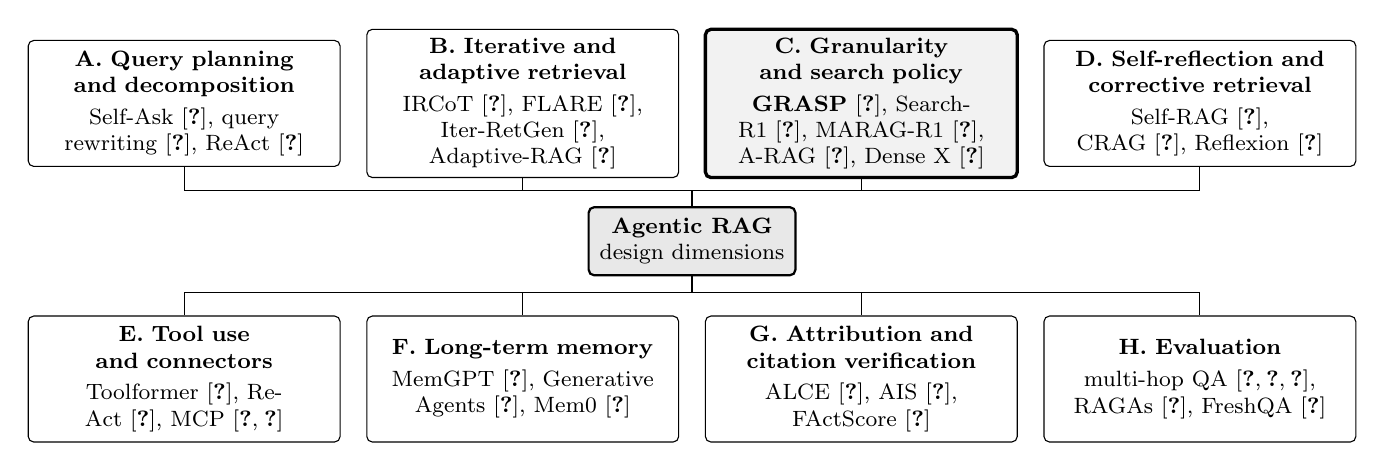
\begin{tikzpicture}[
  font=\footnotesize,
  root/.style={draw, thick, rounded corners=2pt, fill=gray!18, align=center, inner sep=4pt, minimum height=7mm},
  cat/.style={draw, rounded corners=2pt, align=center, text width=3.75cm, minimum height=1.6cm, inner sep=3pt},
  hl/.style={cat, very thick, fill=gray!10}
]
\node[root] (root) at (0,0) {\textbf{Agentic RAG}\\design dimensions};
% upper row
\node[cat] (a) at (-6.45, 1.75) {\textbf{A. Query planning and decomposition}\\[2pt] Self-Ask~\cite{press2023selfask}, query rewriting~\cite{ma2023rewrite}, ReAct~\cite{yao2023react}};
\node[cat] (b) at (-2.15, 1.75) {\textbf{B. Iterative and adaptive retrieval}\\[2pt] IRCoT~\cite{trivedi2023ircot}, FLARE~\cite{jiang2023flare}, Iter-RetGen~\cite{shao2023iterretgen}, Adaptive-RAG~\cite{jeong2024adaptiverag}};
\node[hl]  (c) at ( 2.15, 1.75) {\textbf{C. Granularity and search policy}\\[2pt] \textbf{GRASP}~\cite{gandhi2026grasp}, Search-R1~\cite{jin2025searchr1}, MARAG-R1~\cite{luo2025maragr1}, A-RAG~\cite{du2026arag}, Dense X~\cite{chen2024densex}};
\node[cat] (d) at ( 6.45, 1.75) {\textbf{D. Self-reflection and corrective retrieval}\\[2pt] Self-RAG~\cite{asai2024selfrag}, CRAG~\cite{yan2024crag}, Reflexion~\cite{shinn2023reflexion}};
% lower row
\node[cat] (e) at (-6.45,-1.75) {\textbf{E. Tool use and connectors}\\[2pt] Toolformer~\cite{schick2023toolformer}, ReAct~\cite{yao2023react}, MCP~\cite{anthropic2024mcp,hou2025mcp}};
\node[cat] (f) at (-2.15,-1.75) {\textbf{F. Long-term memory}\\[2pt] MemGPT~\cite{packer2023memgpt}, Generative Agents~\cite{park2023generative}, Mem0~\cite{chhikara2025mem0}};
\node[cat] (g) at ( 2.15,-1.75) {\textbf{G. Attribution and citation verification}\\[2pt] ALCE~\cite{gao2023alce}, AIS~\cite{rashkin2023ais}, FActScore~\cite{min2023factscore}};
\node[cat] (h) at ( 6.45,-1.75) {\textbf{H. Evaluation}\\[2pt] multi-hop QA~\cite{yang2018hotpotqa,ho2020twowiki,trivedi2022musique}, RAGAs~\cite{es2024ragas}, FreshQA~\cite{vu2024freshllms}};
% connectors (bus lines)
\draw (root.north) -- (0,0.65);
\draw (-6.45,0.65) -- (6.45,0.65);
\foreach \nd/\x in {a/-6.45,b/-2.15,c/2.15,d/6.45} { \draw (\x,0.65) -- (\nd.south); }
\draw (root.south) -- (0,-0.65);
\draw (-6.45,-0.65) -- (6.45,-0.65);
\foreach \nd/\x in {e/-6.45,f/-2.15,g/2.15,h/6.45} { \draw (\x,-0.65) -- (\nd.north); }
\end{tikzpicture}
\caption{Taxonomy of agentic RAG used in this review. The highlighted branch (C) contains the anchor work, GRASP~\cite{gandhi2026grasp}. Cited methods are representative, not exhaustive, and several appear in more than one branch.}
\label{fig:taxonomy}
\end{figure*}

\subsection{Query Planning and Decomposition}
Planning methods turn one question into a sequence or set of simpler ones. Self-Ask prompts the model to pose and answer explicit follow-up questions, and this structure makes it easy to send each follow-up to a search engine~\cite{press2023selfask}. Rewrite-Retrieve-Read inserts a query-rewriting step before retrieval and trains a small rewriter with RL from the reader's feedback~\cite{ma2023rewrite}. ReAct does not plan up front; it decides the next action after each observation~\cite{yao2023react}. The trade-off is between \emph{plan-then-execute}, which is predictable and easy to run in parallel, and \emph{step-wise} planning, which can adapt to what was found but costs more LLM calls and is harder to bound.

\subsection{Iterative and Adaptive Retrieval}
IRCoT alternates retrieval with chain-of-thought steps: each new reasoning sentence becomes the next query, and the retrieved passages feed the next sentence~\cite{trivedi2023ircot}. FLARE retrieves only when the model's draft of the next sentence contains low-confidence tokens, then regenerates that sentence~\cite{jiang2023flare}. Iter-RetGen feeds a whole draft answer back as the next retrieval query~\cite{shao2023iterretgen}. Adaptive-RAG trains a small classifier to estimate question complexity and routes each query to no retrieval, single-step retrieval or multi-step retrieval~\cite{jeong2024adaptiverag}. These methods decide \emph{when} and \emph{how often} to retrieve, but they keep one retriever and one chunk size.

\subsection{Search Granularity and Search Policies}
\label{sec:grasp}
A newer line of work treats the retrieval interface itself as an action space. Search-R1 trains an LLM with RL to issue search calls during reasoning, using an outcome reward and masking retrieved tokens out of the loss~\cite{jin2025searchr1}. Search-o1 inserts agentic search into the reasoning of large reasoning models~\cite{li2025searcho1}. MARAG-R1 gives the agent four retrieval tools (semantic search, keyword search, filtering and aggregation) and trains it with supervised fine-tuning followed by RL~\cite{luo2025maragr1}. A-RAG exposes hierarchical retrieval interfaces (keyword search, semantic search and chunk reading) that the model combines on its own~\cite{du2026arag}. GRASP is the anchor of this review, and we describe it in detail.

\subsubsection{Problem}
Gandhi \textit{et al.} identify three difficulties in agentic RAG~\cite{gandhi2026grasp}: using lexical and semantic signals together, choosing a context granularity that does not fill the window with irrelevant tokens, and training a policy that decides when, where and how to retrieve across steps. They argue that prior RL-trained agents use a single retriever or a fixed, coarse chunk size, which limits how retrieval can adapt during multi-step reasoning.

\subsubsection{Formulation and actions}
GRASP models agentic RAG as a finite-horizon Markov decision process. The state holds the question, the interaction history, the evidence and tools used so far, and the remaining turn budget. Each paragraph in the corpus is split into sentences, and every sentence keeps a pointer to its parent paragraph. At each step the policy writes a reasoning segment and then picks one of four actions: \emph{semantic search} (dense retrieval with a Qwen3-0.6B model), \emph{keyword search} (BM25), \emph{read paragraph}, which returns the full parent paragraph of a retrieved sentence, and \emph{answer}, which ends the episode. Both search actions return the top-$K$ sentences with their parent identifiers and scores ($K=5$ in the experiments). The agent therefore sees short, sentence-level evidence first and pays for a whole paragraph only when it chooses to read one.

\subsubsection{Reward}
The trajectory reward combines four terms:
\begin{equation}
R = R_A + \alpha R_R + \beta R_S + \gamma R_E, \quad (\alpha,\beta,\gamma) = (0.7, 0.15, 0.15).
\label{eq:grasp}
\end{equation}
$R_A$ is token-level F1 between the predicted and gold answers. $R_R$ (grounded reading) is the F1 between the set of paragraphs the agent read and the gold supporting paragraphs, which rewards reading gold evidence and penalises reading distractors. $R_S$ (complementary search) equals 1 only if \emph{both} semantic and keyword search surface at least one gold paragraph during the trajectory. $R_E$ (turn efficiency) is $(T - T_{\text{cur}})/T$ and is paid only when $R_A > 0.5$, so that the agent cannot earn efficiency credit by guessing early. The auxiliary terms sum to at most 1, so answer accuracy remains the main signal. The authors present this weighting as a guard against reward hacking.

\subsubsection{Training and evaluation}
The policy is Qwen2.5-3B-Instruct, fine-tuned with all parameters using Group Relative Policy Optimization (GRPO)~\cite{shao2024deepseekmath}. It trains on the HotpotQA distractor split~\cite{yang2018hotpotqa} for 270 optimisation steps (about 19\% of one epoch), with a budget of at most 10 turns per trajectory. As in Search-R1, retrieved tokens are masked out of the policy loss. Evaluation uses 500 sampled validation questions from each of HotpotQA, 2WikiMultiHopQA and MuSiQue~\cite{yang2018hotpotqa,ho2020twowiki,trivedi2022musique}; the last two measure transfer, since the model never trains on them. Baselines include single-step lexical, semantic and hybrid retrieval (hybrid uses a Qwen3 re-ranker), IRCoT driven by a proprietary model, two public Search-R1 checkpoints (PPO and GRPO), and an untrained ``Base'' agent with GRASP's prompt and tools.

\begin{table}[t]
\centering
\caption{Selected results reported by GRASP~\cite{gandhi2026grasp}: retrieval recall (R) and answer F1 on 500 validation questions per dataset. All numbers are copied from the GRASP paper; we did not re-run them.}
\label{tab:grasp}
\setlength{\tabcolsep}{4pt}
\footnotesize
\begin{tabular}{@{}lcccccc@{}}
\toprule
 & \multicolumn{2}{c}{HotpotQA} & \multicolumn{2}{c}{2Wiki} & \multicolumn{2}{c}{MuSiQue} \\
\cmidrule(lr){2-3}\cmidrule(lr){4-5}\cmidrule(lr){6-7}
Method & R & F1 & R & F1 & R & F1 \\
\midrule
Single-step hybrid   & 0.86 & 0.48 & 0.60 & 0.32 & 0.59 & 0.20 \\
IRCoT                & \textbf{0.91} & 0.36 & 0.83 & 0.40 & 0.62 & 0.15 \\
Search-R1 (PPO)      & 0.76 & 0.47 & 0.74 & 0.48 & 0.55 & 0.26 \\
Search-R1 (GRPO)     & 0.74 & 0.56 & 0.77 & 0.53 & 0.62 & 0.30 \\
Base (no RL)         & 0.36 & 0.24 & 0.27 & 0.20 & 0.24 & 0.10 \\
GRASP                & 0.90 & \textbf{0.66} & \textbf{0.90} & \textbf{0.60} & \textbf{0.70} & \textbf{0.33} \\
\bottomrule
\end{tabular}
\end{table}

\subsubsection{Findings}
Table~\ref{tab:grasp} summarises the main results. GRASP has the best answer F1 on all three datasets and the best recall on 2WikiMultiHopQA and MuSiQue. IRCoT has slightly higher recall on HotpotQA, which the authors attribute to the strong proprietary model that writes its reasoning. They also note that IRCoT scores well under an LLM judge but lower on exact match and F1. The untrained Base agent does much worse than even single-step retrieval. This shows that giving a small model more tools does not help unless it also learns how to use them. An ablation trained on a 5{,}500-question HotpotQA subset is especially relevant to granularity. Removing keyword search lowers F1 only slightly (0.631 to 0.621). Removing semantic search lowers it more (0.567). Removing the read action, so that both searches return whole paragraphs, causes the largest drop (0.484). The authors observe that with paragraph-level results the agent writes follow-up queries that stay close to the original question, because a paragraph exposes many entities at once and gives a weaker signal about which clue to pursue next.

\subsubsection{Learned behaviour}
A first-order Markov analysis of the trained agent's action sequences shows a regular pattern. The agent starts with semantic search to locate the topic, reads a paragraph to confirm local context and extract a bridge entity, and then runs keyword search on that entity. If the keyword search returns nothing useful, it goes back to a broader semantic query. The authors compare this to human skimming and scanning.

\subsubsection{Limitations stated by the authors}
$R_R$ and $R_S$ need gold supporting-fact annotations, which few corpora provide. The policy still sometimes answers before the needed evidence has appeared. Only one 3B backbone was tested, and tool use settles at about eight calls per trajectory. For future work the authors propose richer tool spaces, rewards built from weaker or model-based grounding signals, and fully dynamic granularity from spans up to larger document regions. Their ethics statement also recommends provenance tracking, citations, audit logs and human approval for consequential actions. Several of these recommendations reappear in Section~\ref{sec:cortex}.

\subsection{Self-Reflection and Corrective Retrieval}
Self-RAG trains one model to emit reflection tokens that decide whether to retrieve and whether a passage is relevant to, and supports, the output~\cite{asai2024selfrag}. CRAG adds a lightweight evaluator that scores retrieved documents. When retrieval looks wrong, CRAG falls back to web search, and it filters documents by splitting them into strips and recombining the useful ones~\cite{yan2024crag}. Reflexion stores verbal feedback from failed attempts in an episodic buffer and uses it on the next attempt~\cite{shinn2023reflexion}. These methods move quality control inside the loop. GRASP has no explicit critic; instead, its grounded-reading reward shapes what the policy reads during training.

\subsection{Tool Use and Connector Protocols}
Agentic RAG over real data needs connectors to many systems, each with its own API and authentication. Toolformer and ReAct established the tool-calling pattern~\cite{schick2023toolformer,yao2023react}. The Model Context Protocol (MCP), introduced by Anthropic in November 2024, standardises how an application finds and calls tools and resources exposed by external servers~\cite{anthropic2024mcp}. MCP makes adding a connector a configuration change rather than new code. It also widens the attack surface: Hou \textit{et al.} describe a server lifecycle and a taxonomy of threats against MCP deployments~\cite{hou2025mcp}. Indirect prompt injection, where retrieved content contains instructions aimed at the model, is a direct risk once retrieved text can trigger tool calls~\cite{greshake2023injection}.

\subsection{Long-Term Memory}
MemGPT treats the context window like main memory in an operating system and pages information to and from external storage through function calls~\cite{packer2023memgpt}. Generative Agents keep a memory stream and retrieve from it by recency, importance and relevance, with periodic reflection that writes higher-level summaries back into memory~\cite{park2023generative}. Mem0 extracts, consolidates and retrieves salient facts from conversations, with a graph-based variant~\cite{chhikara2025mem0}. For RAG over personal data, memory is both useful (stated priorities can re-weight an answer) and risky (stored facts may be stale, wrong or private), so governance (provenance, expiry, deletion) becomes a design question in its own right.

\subsection{Attribution and Citation Verification}
ALCE introduced a benchmark and automatic metrics for LLM answers with citations, and found that even strong models often lack full citation support~\cite{gao2023alce}. The AIS framework defines when a statement is ``attributable to identified sources'' and gives a human annotation protocol~\cite{rashkin2023ais}. FActScore splits long outputs into atomic facts and checks each against a knowledge source~\cite{min2023factscore}. These works argue for verification at the level of individual claims rather than whole answers, which is the approach Cortex takes.

\subsection{Evaluation}
Most agentic RAG papers, GRASP included, evaluate on Wikipedia-based multi-hop QA with gold supporting paragraphs~\cite{yang2018hotpotqa,ho2020twowiki,trivedi2022musique}. RAGAs offers reference-free metrics for faithfulness and relevance~\cite{es2024ragas}, and FreshQA targets questions whose answers change over time~\cite{vu2024freshllms}. There is still little shared evaluation for agents that work over private, changing, multi-source data and that can also act.

%=====================================================================
\section{Comparative Analysis}
\label{sec:compare}
%=====================================================================

Table~\ref{tab:compare} compares representative methods. ``Granularity'' records whether the evidence unit is fixed or chosen by the agent. ``Live'' records whether the method was \emph{designed for} sources that change at query time, as opposed to a fixed index. Entries describe each method as published; ``--'' means the dimension is not a focus of that work, not that it would be impossible to add.

\begin{table*}[t]
\centering
\caption{Comparison of surveyed methods and the Cortex case study along the taxonomy dimensions.}
\label{tab:compare}
\scriptsize
\setlength{\tabcolsep}{3pt}
\renewcommand{\arraystretch}{1.12}
\begin{tabular}{@{}p{1.55cm}p{3.05cm}p{2.05cm}p{2.0cm}p{1.75cm}p{2.25cm}p{1.75cm}p{1.6cm}@{}}
\toprule
\textbf{Method} & \textbf{Retrieval strategy} & \textbf{Granularity control} & \textbf{Policy} & \textbf{Memory} & \textbf{Verification / critique} & \textbf{Live data} & \textbf{Actions} \\
\midrule
RAG~\cite{lewis2020rag} & Single-shot dense retrieval & Fixed passage & Fine-tuned retriever and generator & -- & -- & -- & -- \\
Self-Ask~\cite{press2023selfask} & Explicit follow-up sub-questions & Search-engine answers & Prompting & -- & -- & Web search & -- \\
IRCoT~\cite{trivedi2023ircot} & Retrieve at each reasoning step & Fixed paragraph & Prompting & -- & -- & -- & -- \\
FLARE~\cite{jiang2023flare} & Retrieve when draft has low confidence & Fixed passage & Prompting & -- & Regenerate uncertain sentence & -- & -- \\
Adaptive-RAG~\cite{jeong2024adaptiverag} & Route: none / single / multi-step & Fixed & Trained classifier & -- & -- & -- & -- \\
Self-RAG~\cite{asai2024selfrag} & On-demand via reflection tokens & Fixed passage & Fine-tuned & -- & Relevance and support tokens & -- & -- \\
CRAG~\cite{yan2024crag} & Evaluator-triggered correction & Strip filtering & Trained evaluator & -- & Retrieval evaluator & Web fallback & -- \\
ReAct~\cite{yao2023react} & Interleaved thought and action & API page / lookup & Prompting & -- & -- & Wikipedia API & Environment actions \\
Search-R1~\cite{jin2025searchr1} & Multi-turn search in reasoning & Fixed passage & RL (PPO, GRPO) & -- & -- & -- & -- \\
MARAG-R1~\cite{luo2025maragr1} & Semantic, keyword, filter, aggregate tools & Fixed chunk & SFT then RL & -- & -- & -- & -- \\
A-RAG~\cite{du2026arag} & Hierarchical retrieval interfaces & Keyword to chunk & Model-driven tool use & -- & -- & -- & -- \\
\textbf{GRASP}~\cite{gandhi2026grasp} & Semantic and keyword search, coordinated & Sentence, expand to paragraph on demand & RL (GRPO), 4-part reward & -- & Grounded-reading reward (training only) & -- & -- \\
MemGPT~\cite{packer2023memgpt} & Paging between context and storage & -- & Function calls & Tiered virtual context & -- & -- & -- \\
Mem0~\cite{chhikara2025mem0} & Memory extraction and retrieval & -- & -- & Consolidated, graph variant & -- & -- & -- \\
\midrule
\textbf{Cortex} (ours) & LLM plan of 2--5 sub-questions, parallel per-source search, one bounded retry & Fixed per source item & Prompted planner, hard budgets; no learning & Salience, TTL, decay, pin/edit/forget & Claim-level lexical check, LLM re-check, conflicts & Mail, calendar, docs, chat, code, web, MCP & Proposed; run only after consent \\
\bottomrule
\end{tabular}
\end{table*}

Three patterns stand out. First, learned search policies (Search-R1, MARAG-R1, GRASP) have so far been studied on static, Wikipedia-derived corpora with gold evidence, while systems built for live data mostly rely on prompting. Second, granularity is chosen by the agent at query time only in recent work (A-RAG, GRASP); GRASP's ablation is, to our knowledge, the clearest evidence that this choice changes answer quality. Third, memory, claim verification and actions are rarely combined with learned retrieval. They are system-level concerns that appear mainly in deployed agents, where trust, cost and side effects matter more than benchmark accuracy.

%=====================================================================
\section{Case Study: Cortex}
\label{sec:cortex}
%=====================================================================

Cortex answers questions such as ``what changed in this project this week, and what is at risk?'' over a user's connected sources. It returns an answer in which factual sentences cite numbered evidence, flags claims it could not verify, and lists contradictions between sources. When the user asks it to do something, it drafts an action and waits for approval. The description below follows the source code (TypeScript agent, connector and LLM packages, and a Python memory service), not the project's roadmap.

\subsection{Architecture}
Fig.~\ref{fig:cortex} shows one run. The orchestrator is a hand-written, bounded loop rather than a graph framework, so that every branch is explicit and the number of LLM calls is predictable. Hard limits apply to every run: at most 5 sub-questions, 18 tool calls, 4 LLM calls in Deep mode (2 in Fast mode), 16 evidence items (8 in Fast mode) and 90\,s in total.

\begin{figure}[t]
\centering
\resizebox{\columnwidth}{!}{%
\begin{tikzpicture}[
  font=\scriptsize,
  step/.style={draw, rounded corners=2pt, align=center, text width=3.3cm, minimum height=6.5mm, inner sep=2pt, fill=white},
  side/.style={draw, dashed, rounded corners=2pt, align=center, text width=2.35cm, inner sep=2pt},
  gate/.style={draw, very thick, rounded corners=2pt, align=center, text width=2.35cm, inner sep=2pt, fill=gray!12},
  arr/.style={-{Stealth[length=1.5mm]}},
  darr/.style={{Stealth[length=1.5mm]}-{Stealth[length=1.5mm]}}
]
\node[step] (u) at (0, 0)   {\textbf{Understand}: check which sources are live; report outages};
\node[step] (r) at (0,-1)   {\textbf{Recall}: top memories (pinned always included)};
\node[step] (p) at (0,-2)   {\textbf{Plan} (LLM, JSON): intent, time window, 2--5 sub-questions with sources and keywords};
\node[step] (s) at (0,-3.1) {\textbf{Search}: all (sub-question $\times$ source) pairs in parallel; dedupe; rank by keyword hits and recency};
\node[step] (y) at (0,-4.25) {\textbf{Synthesize} (LLM, streamed): cite every fact; list conflicts, gaps, actions};
\node[step] (v) at (0,-5.3) {\textbf{Verify}: lexical claim check; LLM re-check of doubtful claims};
\node[step] (a) at (0,-6.3) {\textbf{Propose actions}: validate against connector schema; never execute};
\node[step] (m) at (0,-7.3) {\textbf{Remember}: explicit requests, or salient candidates ($\geq 0.6$)};
\foreach \x/\y in {u/r, r/p, p/s, s/y, y/v, v/a, a/m} { \draw[arr] (\x) -- (\y); }
% left: memory service spanning recall..remember
\node[side, minimum height=7.0cm, text width=1.55cm] (mem) at (-3.0,-4.15) {\textbf{Memory service}\\[2pt] vector search or SQLite FTS5\\[2pt] provenance, TTL, decay, pin, forget};
\draw[darr] (r.west) -- (r.west -| mem.east);
\draw[arr] (m.west) -- (m.west -| mem.east);
% right: connectors, router, consent gate
\node[side] (c) at (3.25,-3.1) {\textbf{Connectors}: Composio (6 apps), MCP servers, Firecrawl web, sample workspace};
\node[side, minimum height=1.55cm] (l) at (3.25,-4.78) {\textbf{LLM router}: free-tier providers, failover, cooldowns, response cache};
\node[gate] (g) at (3.25,-6.3) {\textbf{User consent}: approve / edit / decline; single-use, 30\,min expiry};
\draw[darr] (s.east) -- (s.east -| c.west);
\draw[arr] (y.east) -- (y.east -| l.west);
\draw[arr] (v.east) -- (v.east -| l.west);
\draw[arr] (a.east) -- (a.east -| g.west);
\draw[arr, dashed] (g.north east) .. controls +(0.5,0.6) and +(0.6,-0.6) .. node[right, align=left, font=\tiny] {execute\\once} (c.south east);
\end{tikzpicture}%
}
\caption{One Cortex run in Deep mode. If search returns no evidence, the run stops after \emph{Search} and Cortex reports what it searched without making an LLM call. Execution happens only on a separate approval request.}
\label{fig:cortex}
\end{figure}

\textbf{Understand and recall.} The registry asks each connector for its status. A source that is down produces an event that names the source, the reason (for example, an expired connection) and its \emph{impact} on the answer, and the run continues without it. Memories are retrieved next. Pinned memories are always included; the rest are ranked by relevance weighted by salience.

\textbf{Plan.} In Deep mode one LLM call returns JSON with an intent (research, action or chat), a rewritten question that resolves references from the conversation, an optional time window, and 2--5 sub-questions. Each sub-question names 1--3 sources and a short keyword query. The plan is validated against the connected sources. If the output is unusable, Cortex falls back to a single sub-question over all sources with a locally parsed time window, which is also the plan used in Fast mode.

\textbf{Search and rank.} Every unique (source, query) pair runs in parallel. Each connector call has a 12\,s timeout, one retry for transient errors and a 90\,s result cache. In Deep mode, sub-questions that found nothing get one broadened retry (fewer keywords, no time window) without an extra LLM call. Evidence is deduplicated and ranked by keyword overlap with a small recency bonus. If nothing is found, Cortex says which sources it searched and does not guess. This path costs no LLM call.

\textbf{Synthesize.} The model may use only the numbered evidence and must cite each factual sentence. After the answer it writes five machine-readable sections: conflicts between sources, parts of the question that the evidence does not cover, proposed actions (JSON), memory candidates (JSON) and follow-up questions.

\textbf{Verify.} Each sentence is checked against the evidence it cites. A cited claim is \emph{supported} if at least 40\% of its content words appear in the cited evidence and every number it states appears there too, \emph{partial} at 20\% overlap, and \emph{unsupported} otherwise. An uncited factual sentence is unsupported unless it closely matches the evidence of the sentence before it, and hedging sentences are skipped. In Deep mode, up to eight doubtful claims that do cite evidence are re-checked by one LLM call. Groundedness is the mean claim score, with partial support counted as half. The interface strikes through unsupported claims and shows conflicts with both citations.

\textbf{Actions.} Proposed actions are checked against the connector's action schema (the action must exist and required parameters must be present). Each valid proposal is stored on the server with an exact, human-readable preview and shown as a confirmation card. Only the approval endpoint calls the connector's execute method. Each approval is tied to one user, can be used once and expires after 30 minutes.

\textbf{Memory.} Cortex, not the memory backend, decides what to keep. Automatic extraction in the memory library is turned off. Explicit requests (``remember that\ldots'') are stored with salience 0.95; model-proposed facts are stored only at salience $\geq 0.6$, at most two per run. Each kind of memory has a time-to-live (for example, 45 days for priorities and 90 for facts; preferences do not expire). Salience decays with a 30-day half-life unless the memory is pinned, and a near-duplicate reinforces an existing memory instead of creating a new one. Users can pin, edit or delete memories. Search uses Oracle Agent Memory's vector index when it is configured and SQLite FTS5 (BM25) otherwise.

\textbf{Connectors and models.} Six workspace apps (Gmail, Google Calendar, Google Drive, Notion, Slack and GitHub) are reached through Composio with managed OAuth. Any MCP server, over HTTP or stdio, can be added through a configuration file. Firecrawl provides web search, and a fictional sample workspace with deliberate cross-source conflicts supports demos and evaluation. Tool outputs of any shape are mapped to a common evidence record (title, quote, URL, author, timestamp). An LLM router sends requests to OpenAI-compatible free-tier providers in order (Groq, Gemini, Cerebras, OpenRouter, with Puter as a last resort). It applies per-provider cooldowns after rate-limit or key errors, caches responses, and fails over a streamed answer only before the first token arrives.

\subsection{Mapping Cortex to the Literature}
Table~\ref{tab:map} links each design choice to the work it draws on and states how GRASP relates to it.

\begin{table}[t]
\centering
\caption{Cortex design choices, related work and relation to GRASP.}
\label{tab:map}
\scriptsize
\setlength{\tabcolsep}{3pt}
\renewcommand{\arraystretch}{1.12}
\begin{tabular}{@{}p{1.6cm}p{1.95cm}p{4.3cm}@{}}
\toprule
\textbf{Cortex choice} & \textbf{Related work} & \textbf{Relation to GRASP} \\
\midrule
Up-front plan of sub-questions & Self-Ask~\cite{press2023selfask}, rewriting~\cite{ma2023rewrite} & GRASP decides step by step; Cortex plans once for predictable cost. \\
Parallel search, one retry & IRCoT~\cite{trivedi2023ircot}, Adaptive-RAG~\cite{jeong2024adaptiverag} & GRASP-style multi-turn search could replace the fixed retry when a hop depends on an earlier result. \\
Item-level evidence & Dense X~\cite{chen2024densex}, A-RAG~\cite{du2026arag} & Fixed granularity; GRASP's ablation suggests adding sentence hits with an explicit ``read'' action. \\
Keyword queries to native source search & BM25~\cite{robertson2009bm25}, DPR~\cite{karpukhin2020dpr} & Single signal per source; GRASP's complementary-search idea applies. \\
Hard budgets & FLARE~\cite{jiang2023flare}, Adaptive-RAG~\cite{jeong2024adaptiverag} & Analogous to GRASP's turn-efficiency term, but fixed rather than learned. \\
Claim verification, conflicts & ALCE~\cite{gao2023alce}, AIS~\cite{rashkin2023ais}, FActScore~\cite{min2023factscore}, CRAG~\cite{yan2024crag} & Could supply the weak grounding signal GRASP lists as future work. \\
Honest ``not found'', missing list & Self-RAG~\cite{asai2024selfrag} & Targets GRASP's stated failure mode of premature answers. \\
Governed memory & MemGPT~\cite{packer2023memgpt}, Gen.\ Agents~\cite{park2023generative}, Mem0~\cite{chhikara2025mem0} & Outside GRASP's scope. \\
MCP connectors, consent gate & ReAct~\cite{yao2023react}, MCP~\cite{anthropic2024mcp,hou2025mcp}, injection~\cite{greshake2023injection} & Follows GRASP's ethics advice on human approval for consequential actions. \\
\bottomrule
\end{tabular}
\end{table}

\textbf{Planning and retrieval.} Cortex's planner is close to Self-Ask and query rewriting: it writes the sub-questions up front and sends a keyword query for each to the sources it names~\cite{press2023selfask,ma2023rewrite}. This is a deliberate trade-off. One planning call and one synthesis call fit within free-tier rate limits, and parallel search keeps latency low. The cost is that a sub-question cannot use what an earlier one found, which is exactly the bridge-entity pattern that IRCoT and GRASP exploit~\cite{trivedi2023ircot,gandhi2026grasp}. The single broadened retry is a fixed heuristic for one failure case (empty results) and is not an adaptive policy.

\textbf{Where GRASP applies.} Four GRASP ideas map directly onto Cortex. (i) \emph{Read on demand.} Cortex currently passes each source item's quote to the synthesizer as one unit. A long email thread or design document therefore enters the context whole or truncated. GRASP's results suggest a different design: return the best-matching sentences with a pointer to the parent item, and let the agent ``read'' the full thread only when a snippet is promising but incomplete. (ii) \emph{Complementary signals.} Each Cortex connector uses the source's own search, which is mostly keyword-based. An embedding index over recently fetched items could provide a second, semantic signal. GRASP's ablation shows that the semantic signal mattered more on its benchmarks, although that result may not hold for workspace data, where identifiers such as issue numbers and names are common. (iii) \emph{Learned budgets.} Cortex's hard limits play the role of GRASP's turn-efficiency term but cannot adapt to how hard a question is. (iv) \emph{Weak rewards.} GRASP's grounded-reading and complementary-search rewards need gold supporting paragraphs. Cortex has none, but its verifier assigns each claim a support label tied to specific evidence. Such labels could serve as the model-based grounding signal that the GRASP authors propose for corpora without annotations. Training a policy this way would require care, since a policy could learn to satisfy a lexical verifier without becoming more correct.

\textbf{Where Cortex goes beyond GRASP's setting.} GRASP studies a static, single-domain Wikipedia corpus. Cortex has to handle problems that this setting does not raise. Its sources fail independently, so it reports outages and their impact. Facts carry timestamps and change, so it filters by time window and gives a recency bonus. Sources can contradict each other, so it surfaces conflicts instead of choosing one. Finally, it can change external state, so execution is separated from the model's output and gated by explicit user consent, a safeguard that matters given indirect prompt injection through retrieved content~\cite{greshake2023injection,hou2025mcp}.

\subsection{Preliminary Measurements}
Cortex includes a 12-question evaluation over its fictional sample workspace. The run reported here used Deep mode with free-tier models. Groq's \texttt{openai/gpt-oss-120b} was the primary strong model and Gemini 3.5 Flash-Lite the fallback; the smaller fast-tier model handled planning and claim re-checks, and other free-tier providers were available for failover. Table~\ref{tab:prelim} lists the results. Groundedness is the verifier's mean claim score described above. Citation recall is the fraction of expected key facts for each question that appear in the cited evidence, averaged over questions.

\begin{table}[t]
\centering
\caption{Preliminary Cortex measurements (12 questions, fictional sample workspace, free-tier models, single run). These are not a benchmark comparison.}
\label{tab:prelim}
\footnotesize
\begin{tabular}{@{}lr@{}}
\toprule
Metric & Value \\
\midrule
Mean groundedness (lexical check + LLM re-check) & 0.88 \\
Mean citation recall & 0.92 \\
Honest ``not found'' answers & 1/1 \\
Cross-source conflicts detected & 1/2 \\
Expected actions proposed & 1/2 \\
Actions executed without explicit consent & 0 \\
Median latency & 3.7\,s \\
90th-percentile latency & 7.1\,s \\
\bottomrule
\end{tabular}
\end{table}

These numbers should be read with care. The question set is small and was written by the developers. The workspace is synthetic. Groundedness is measured by Cortex's own verifier, which is partly lexical and may both over-credit paraphrases and under-credit correct inferences. No other system was run on the same data, so the results cannot be compared with GRASP or any other method. Within these limits, the run supports three observations: the citation and verification path works end to end, the system did not invent an answer when the evidence was absent, and the consent gate held. It also points to weaknesses. Conflict detection and action proposals each succeeded on only one of two cases, and both depend on the synthesizer noticing the issue, not on a dedicated component.

%=====================================================================
\section{Open Challenges and Future Directions}
\label{sec:challenges}
%=====================================================================

\textbf{Supervision without gold evidence.} RL-trained search policies, GRASP included, rely on rewards computed from gold supporting facts~\cite{gandhi2026grasp,luo2025maragr1}. Private and live corpora have no such labels. Promising substitutes include verifier-based support labels, agreement across sampled trajectories, and attribution scores in the spirit of AIS and FActScore~\cite{rashkin2023ais,min2023factscore}. Each of these can be gamed, so reward design needs held-out human checks.

\textbf{Granularity over heterogeneous data.} Sentences and paragraphs are natural units for Wikipedia. For an email thread, a pull request with review comments, a calendar event or a table in a document, the right ``sentence'' and ``parent'' are less obvious. Hierarchical units~\cite{sarthi2024raptor,du2026arag} and propositions~\cite{chen2024densex} suggest options, but how agents should move between levels in structured, multi-source data is still an open question.

\textbf{Freshness, time and conflict.} Benchmarks such as FreshQA show that time-sensitive questions remain hard~\cite{vu2024freshllms}. Agents over live data must reason about when a fact was true, which source is authoritative, and when to report disagreement rather than resolve it. Few methods treat conflict as an output instead of noise.

\textbf{Verification quality.} Lexical overlap is cheap but crude. LLM judges are more flexible but cost calls and can be wrong in their own ways. Claim-level checking should be calibrated against human judgements of attribution~\cite{rashkin2023ais,gao2023alce}, and verifiers should report uncertainty instead of a single score.

\textbf{Safety of acting agents.} Once retrieved text can lead to tool calls, indirect prompt injection becomes a practical threat~\cite{greshake2023injection}, and connector protocols add their own attack surface~\cite{hou2025mcp}. Consent gates, least-privilege connectors, exact previews and audit logs are necessary but not sufficient. A systematic evaluation of agentic RAG under adversarial content is still missing.

\textbf{Memory governance.} Long-term memory improves personalisation~\cite{packer2023memgpt,park2023generative,chhikara2025mem0}, but it raises questions of consent, staleness and deletion. Explainable memory, which records why an item was kept and where it came from and supports expiry and user deletion, is a design direction that current benchmarks do not measure.

\textbf{Cost-aware policies.} Learned policies reach about eight tool calls per question in GRASP~\cite{gandhi2026grasp}, and deployed systems on free tiers must also budget LLM calls. Future policies could learn when to stop under explicit cost and latency constraints and could work with routing across model sizes, as Adaptive-RAG does for retrieval depth~\cite{jeong2024adaptiverag}.

\textbf{Evaluation for live, multi-source agents.} Shared benchmarks for agents over private, changing data are lacking, and so are protocols that score not only answer accuracy but also citation support, honest abstention, conflict reporting and the safety of proposed actions. Synthetic workspaces with seeded conflicts, like the one used for Cortex, are a small step; reproducible versions with time-stamped snapshots and larger question sets would make results comparable across systems.

%=====================================================================
\section{Conclusion}
%=====================================================================

Agentic RAG has moved from fixed retrieve-then-read pipelines to agents that plan, search repeatedly, critique evidence, use tools and remember. GRASP adds an important point to this picture: the \emph{amount} of context an agent reads, and the retrieval signal it uses to find it, are decisions worth learning. On its benchmarks, a small model trained to read sentence-level hits and expand to paragraphs only when needed outperformed prompting-based and RL-based baselines on answer F1. Our case study shows a different part of the design space. Cortex works over live, heterogeneous sources under tight cost limits and puts its effort into claim verification, conflict reporting, governed memory and consent-gated actions, while keeping a simple, fixed retrieval plan. The two approaches complement each other. Bringing granularity-aware, learned search into systems like Cortex will require rewards that do not depend on gold evidence, evidence units suited to mail, chat and code, and evaluations that also measure trust and safety, not only accuracy.

\bibliographystyle{IEEEtran}
\bibliography{refs}

\end{document}
